%
% chapter.tex -- Kapitel zu partiellen Differentialgleichungen
%
% (c) 2021 Prof Dr Andreas Müller, OST Ostschweizer Fachhochschule
%
% !TeX spellcheck = de_CH
\chapter{Partielle Differentialgleichungen
\label{buch:chapter:pde}}
\lhead{Partielle Differentialgleichungen}
\rhead{}
Partielle Differentialgleichungen sind eine besonders ergiebige
Quelle für Anwendungen spezieller Funktionen.
Die Separationsmethode zum Beispiel für die Wellengleichung
auf gewissen, besonders einfachen Gebieten wie Rechtecken,
Kreisscheiben oder Kugel führt auf gewöhnliche Differentialgleichungen,
deren Lösungen spezielle Funktionen sind.

%
% gleichung.tex
%
% (c) 2021 Prof Dr Andreas Müller, OST Ostschweizer Fachhochschule
%
\section{Gleichungen und Randbedingungen
\label{buch:pde:section:gleichungen-und-randbedingungen}}
\rhead{Gebiete, Gleichungen und Randbedingungen}

\subsection{Gebiete, Differentialoperatoren, Randbedingungen}


\subsubsection{Gebiete}
Gewöhnliche Differentialgleichungen haben nur eine unabhängige
Variable, die gesuchte Lösungsfunktion ist auf eine 
Intervall in $\mathbb{R}$ definiert.
Die Lösungsfunktion einer partiellen Differentialgleichung
ist auf einer Teilmenge von $\mathbb{R}^n$ definiert, des 
ermöglicht wesentlich vielfältigere und kompliziertere
Situationen.

\begin{definition}
Ein Gebiet $G\subset\mathbb{R}^n$ ist eine offene Teilmenge
von $\mathbb{R}^n$, d.~h.~für jeden Punkt $x\in G$ gibt es
eine kleine Umgebung
\(
U_{\varepsilon}(x)
=
\{y\in\mathbb{R}^n\mid |x-y|<\varepsilon\}
\), die ebenfalls in $G$ in enthalten ist,
also $U_{\varepsilon}(x)\subset G$.
\end{definition}

\subsubsection{Differentialoperatoren}
Eine gewöhnliche Differentialgleichung für eine Funktion
ist eine Beziehung zwischen den Werten der Funktion und ihrer
Ableitung in jedem Punkt des Definitionsintervalls.
Eine partielle Differentialgleichung ist entsprechend eine
Beziehung zwischen den Werten einer Funktion und ihren partiellen
Ableitungen.
Eine Funktion von mehreren Variablen hat sehr viel mehr partielle
Ableitungen, bereits partielle Differentialgleichungen erster
Ordnung sind daher sehr viel vielfältiger.
Bei höheren partiellen Ableitungen kommen noch die zusätzliche Bedingungen
\[
\frac{\partial^2 u}{\partial x_i\,\partial x_j}
=
\frac{\partial^2 u}{\partial x_j\,\partial x_i}
\]
hinzu, die für jedes Paar von Indizes $i,j$ ebenfalls erfüllt sein
müssen.

In diesem Kapitel betrachten wir ausschliesslich lineare
Differentialgleichungen.
Die Funktionswerte und partiellen Ableitungen lassen sich daher
in der Form eines Operators
\[
L 
=
a
+ \sum_{i=1}^n b_i \frac{\partial}{\partial x_i}
+ \sum_{i,j=1}^n c_{ij} \frac{\partial^2}{\partial x_i\,\partial x_j}
+ \dots
\]
schreiben.
Die Koeffizienten $a$, $b_i$, $c_{ij}$ können dabei durchaus auch
Funktionen der unabhängigen Variablen sein.

\subsubsection{Laplace-Operator}
Der Laplace-Operator hat in einem karteischen Koordinatensystem die
Form
\[
\Delta
=
\frac{\partial^2}{\partial x_1^2}
+
\frac{\partial^2}{\partial x_2^2}
+
\dots
+
\frac{\partial^2}{\partial x_n^2}.
\]
Er zeichnet sich durch die Eigenschaft aus, dass eine beliebige 
Translation oder Drehung des Koordinatensystems den Wert von $\Delta u$
nicht ändert.
Man könnte sagen, der Laplace-Operator ist symmetrisch bezüglich
aller Bewegungen des Raumes.

\subsubsection{Wellengleichung}

\subsubsection{Eigenfunktionen}
Eine besonders einfache 

\subsubsection{Trigonometrische Funktionen}
Die trigonometrischen Funktionen 

\subsection{Orthogonalität}
In der linearen Algebra lernt man, dass die Eigenvektoren einer
symmetrischen Matrix zu verschiedenen Eigenwerten orthgonal sind.
Dies hat zur Folge, dass die Transformation in eine Eigenbasis
mit einer orthogonalen Matrix möglich ist, was wiederum die Basis
von Diagonalisierungsverfahren wie dem Jacobi-Verfahren ist.

Das Separationsverfahren wird zeigen, wie sich das Finden einer
Lösung der Wellengleichung auf Lösungen des Eigenwertproblems
$\Delta u = \lambda u$ zurückführen lässt.
Damit stellt sich die Frage, welche Eigenschaften 


\subsubsection{Gewöhnliche Differentialglichung}


\subsubsection{$n$-dimensionaler Fall}

%
% separation.tex
%
% (c) 2021 Prof Dr Andreas Müller, OST Ostschweizer Fachhochschule
%
\section{Separationsmethode
\label{buch:pde:section:separation}}
Die Existenz der Lösung einer gewöhnlichen Differentialgleichung
ist unter einigermassen milden Bedingungen in der Nähe der
Anfangsbedingung garantiert.
Ausserdem steht eine ganze Reihe von Lösungsverfahren zur
Verfügung, nicht zuletzt das Potenzreihenverfahren, welches in
Kapitel~\ref{buch:chapter:differential} beschrieben wurde.
Das Ziel dieses Abschnitts ist eine Methode vorzustellen, mit
der partielle Differentialgleichungen auf gewöhnliche
Differentialgleichungen zurückgeführt werden können.

%
% Ansatz
%
\subsection{Separationsansatz}
Die Separationsmethode ist motiviert durch die Beobachtung, dass in
vielen partiellen Differentialgleichungen die Ableitungen nach
verschiedenen Variablen sich in verschiedenen Termen befinden und
sich daher algebraisch trennen lassen.
Für eine beliebige Funktion bringt das nicht viel, aber für
Funktionen mit einer speziellen Form kann man daraus eine Vereinfachung
ableiten.

%
% Prinzip der Separation
%
\subsubsection{Prinzip}
Die Grundlage der Separationsmethode ist die Idee, die Differentialgleichung
in zwei Teile aufzuteilen, die keine gemeinsamen Variablen enthalten.
Eine partielle Differentialgleichungen in einem zweidimensionalen
Gebiet mit den Koordinaten $x$ und $y$ soll so umgeformt
werden, dass auf der linken Seite des Gleichheitszeichens nur
die Variable $x$ vorkommt und auf der rechten nur die Variable $y$.
Es entsteht also eine Gleichung der Form
\begin{equation}
F(x) = G(y).
\label{buch:pde:ansatz:eqn:F=G}
\end{equation}
Wie so etwas gehen gehen kann wird weiter unten untersucht.

Betrachtet hält man in der Gleichung~\eqref{buch:pde:ansatz:eqn:F=G}
die Variable $x$ fest, steht links eine fest Zahl, schreiben wir 
sie $\lambda$.
Die Gleichung wird also zu
\[
\lambda = G(y),
\]
sie muss für alle $y$ gelten.
Es folgt dann, dass die rechte Seite gar nicht von $y$ abhängen kann.
Für jeden Wert von $y$ muss $G$ den gleichen Wert $\lambda$ geben.

Wenn aber $G$ konstant ist und immer den Wert $\lambda$ ergibt, dann
ist die Gleichung~\eqref{buch:pde:ansatz:eqn:F=G} auch gleichbedeutend
mit der Gleichung
\[
F(x) = \lambda,
\]
$F$ muss also auch konstant sein.

Die algebraische Trennung der beiden Variablen $x$ und $y$ hat also 
zur Folge, dass die beiden Seiten der Gleichung gar nicht varieren
können, beide Seiten müssen konstant sein.
Die Konstante ist allerdings nicht bekannt und muss im Laufe der
weiteren Lösungsschritte der Gleichung bestimmt werden.

Die Überlegungen funktionieren auch für eine grössere Zahl von
Variablen.
Entscheidend ist nur, dass die einen Variablen, zum Beispiel
$x_1,\dots,x_k$, nur auf der linken Seite vorkommen und die anderen,
wir nennen sie $x_{k+1},\dots,x_n$ nur auf der rechten.
Die Gleichung hat dann die Form
\begin{equation}
F(x_1,\dots,x_k)
=
G(x_{k+1},\dots,x_n).
\label{buch:pde:ansatz:eqn:FF=GG}
\end{equation}
Setzt man feste Werte von $x_1,\dots,x_k$ ein, ist die linke Seite
eine Zahl, die wir wieder $\lambda$ nennen können.
Es muss also für alle $x_{k+1},\dots,x_n$ gelten, dass
$G(x_{k+1},\dots,x_n)=\lambda$ ist.
Daher ist $G$ eine Konstante, sie ist gar nicht von den Variablen
abhängig.
Wenn aber die rechte Seite konstant ist, dann muss auch für alle
$x_1,\dots,x_k$ gelten, dass $F(x_1,\dots,x_k)=\lambda$ ist,
die linke Seite kann also auch nicht varieren.

\begin{prinzip}
In einer Gleichung
\[
F(x_1,\dots,x_k) = G(x_{k+1},\dots,x_n),
\]
in der die linke Seite nur von $x_1,\dots,x_k$ abhängt und die
rechte nur von $x_{k+1},\dots,x_n$ müssen beide Seiten konstant sein.
\end{prinzip}

%
% Beispiel zur Erklärung des Separationsvorgehens
%
\subsubsection{Ein Beispiel}
In der Differentialgleichung
\[
x\frac{\partial u}{\partial x}
-
y^2\frac{\partial^2 u}{\partial y^2}
=
y^4
\]
kommen die Ableitungen nach $x$ und $y$ in verschiedenen Termen vor.
Wir versuchen daher, auch die Lösungsfunktion als Summe
\[
u(x,y) = X(x) + Y(y)
\]
von Termen zu schreiben, die nur von jeweils einer Variablen abhängen.
Setzt man dies in die Differentialgleichung ein, erhält man
\[
x\frac{\partial}{\partial x}(X(x)+Y(y))
-y^2\frac{\partial}{\partial y}(X(x)+Y(y))
=
xX'(x) -y^2Y'(y)
=
y^4.
\]
Indem man den Term mit $y$ auf die rechte Seite schafft, findet man
die Gleichung
\[
xX'(x) = y^2Y'(y) + y^4,
\]
in der die Variablen $x$ und $y$ separiert sind.
Es folgt, dass beide Seiten konstant sein müssen, es gibt also eine
Konstante $\lambda$ derart, dass
\[
xX'(x) = \lambda
\qquad\text{und}\qquad
y^2Y''(y) +y^4 = \lambda.
\]
Diese beiden Gleichungen lassen sich als Differentialgleichungen in
der üblicheren Form als
\begin{align*}
X'(x) &= \frac{\lambda}{x}
&&\Rightarrow&
X(x) &= \int \frac{\lambda}{x}\,dx = \lambda \log x + C
\\
Y''(y) &= \frac{\lambda - y^4}{y^2}
&&\Rightarrow&
Y'(y)
&=
\int \frac{\lambda-y^4}{y^2}\,dy
=
-\frac{\lambda}{y}-\frac{y^3}3 + D
\\
&
&&\Rightarrow&
Y(y)
&=
\int Y'(y)\,dy
=
-\lambda \log y - \frac{y^4}{12} +Dy +E
\end{align*}
schreiben und im Falle von $X(x)$ mit einem Integral lösen.
$Y(y)$ benötigt zwei Integrationen, ist aber ansonsten nicht
schwieriger zu bestimmen.

Das Beispiel zeigt, dass ein Separationsansatz ermöglicht, eine
partielle Differntialgleichung in mehrere gewöhnliche Differentialgleichungen
zu zerlegen, eine für jede Variable, und zu lösen.

%
% Anpassung des Ansatzes an die Randbedingungen
%
\subsubsection{Separationsansatz und Randbedingungen}
Die im Beispiel gewählte Aufteilung der Lösungsfunktion in eine
Summe macht es sehr schwierig, Randbedingungen der partiellen
Differentialgleichungen in Randbedingungen der gewöhnlichen
Differentialgleichungen zu übersetzen.

Als Beispiel dieser Schwierigkeit betrachten wir die Differentialgleichung
\[
\Delta u
=
\frac{\partial^2 u}{\partial x^2}
+
\frac{\partial^2 u}{\partial y^2}
=
a u
\]
auf dem Gebiet
$\Omega = [0,a]\times [0,b] = \{(x,y)\in\mathbb{R}^2\mid 0<x<a\wedge 0<y<b\}$
mit den Randwerten $u(x,y)=0$ für Punkte auf dem Rand von $\Omega$.
Genauer:
\[
\begin{aligned}
u(0,y) &= 0,& u(a,y) &= 0&&\text{für $0<y<b$} \\
u(x,0) &= 0,& u(x,b) &= 0&&\text{für $0<x<a$}.
\end{aligned}
\]
Ein Ansatz der Form $u(x,y)=X(x) + Y(y)$ bedeutet für die
Randwerte $u(x,y)=0$, dass auf dem Rand $X(x)=-Y(y)$ gelten muss.
Das bedeutet aber, dass $X(0) = -Y(y)$, $Y$ müsste also konstant
sein.

Ein Produktansatz löst das Problem.
Wir verwenden stattdessen einen Produktansatz
$u(x,y) = X(x)\cdot Y(y)$, wobei die Funktionen $X(x)$ und $Y(y)$
nicht konstant sein sollen.
Die Randbedingungen sind
\[
\begin{aligned}
u(0,y) &= X(0) Y(y) = 0&&\Rightarrow& X(0)&=0\\
u(a,y) &= X(a) Y(y) = 0&&\Rightarrow& X(a)&=0\\
u(x,0) &= X(x) Y(0) = 0&&\Rightarrow& Y(0)&=0\\
u(x,b) &= X(x) Y(b) = 0&&\Rightarrow& Y(b)&=0.
\end{aligned}
\]
Der Produktansatz ermöglicht also, die Randbedingungen für die Funktion
$u(x,y)$ in Randbedingungen für die Funktionen $X(x)$ oder $Y(y)$
umzuwandeln.

%
% Eigenwertprobleme
%
\subsection{Eigenwertproblem
\label{buch:pde:subsection:eigenwertproblem}}
Viele partielle Differentialgleichungen der mathematischen Physik
sind zeitabhängig, aber das räumliche Gebiet, in dem sie 
definiert sind, ist nicht von der Zeit abhängig.
Dies 

\subsubsection{Wellengleichung}
Die Schwingung einer ebenen Membran, die in ein emGebiet
$G\subset\mathbb{R}^n$ eingespannt ist, wird durch die
Wellengleichung
\begin{equation}
\frac{1}{c^2} \frac{\partial^2 u}{\partial t^2} = \Delta u,
\label{buch:pde:separation:wellengleichung}
\end{equation}
beschrieben.
Darin ist $u(t,x)$ die Auslenkung der Membran zur Zeit $t>0$ in einem
Punkt $x\in G$ des Gebietes $G$ ist.
Die Randbedingungen zerfallen in zwei Teile:
\begin{itemize}
\item
Bedingungen, die wiedergeben, dass die Membran in einen 
Rahmen eingespannt und damit unbeweglich ist.
Dies bedeutet, dass $u(t,x)=0$ für alle Zeiten $t>0$ und für 
Randpunkte $x\in\partial G$ von $G$ ist.
\item
Bedingungen, die Auslenkung und Geschwindigkeit der Membran zur
Zeit $t=0$ beschreiben, typischerweise ind er Form
\begin{align*}
u(0,x) = f(x),
\frac{\partial u}{\partial t}(0,x) = g(x)
\end{align*}
wobei $f(x)$ und $g(x)$ Funktionen auf dem Gebiet $G$ sind.
\end{itemize}

In der Zeitableitung auf der linken Seite
von~\eqref{buch:pde:separation:wellengleichung}
kommen die Ortskoordinaten nicht vor und im Laplace-Operator
auf der rechten Seite tritt die Zeit nicht auf.
Es ist daher naheliegend zu versuchen, die Lösung der Differntialgleichung
als Produkt
\[
u(t,x) = T(t) \cdot U(x)
\]
zu schreiben.
Wendet man die Differentialgleichung darauf an, wird daraus die Gleichung
\[
\frac{1}{c^2}
T''(t)\cdot U(x)
=
T(t) \cdot \Delta U(x).
\]
Indem man druch $T(t)$ und $U(x)$ teilt, entsteht die separierte Gleichung
\[
\frac{1}{c^2} \frac{T''(t)}{T(t)}
=
\frac{\Delta U(x)}{U(x)}.
\]
Die linke Seite ist nur von der Zeit abhängig, die rechte nur von den
Ortskoordinaten.
Damit ist die Differentialgleichung separiert und das Problem darauf
reduziert, die gewöhnliche Differentialgleichung 
\[
T''(t) = \lambda T(t)
\]
und die partielle Differentialgleichung
\[
\Delta U(x) = \lambda U(x)
\]
niedrigerer Dimension zu lösen.

\subsubsection{Allgemeine Situation}
Das Definitionsgebiet der partiellen Differentialgleichung ist 
also von der Form $\mathbb{R}^+\times G$, wobei $G\subset\mathbb{R}^n$
ein räumliches Gebiet ist und $\mathbb{R}^+$ die Zeitachse.
Auch die Randbedingungen zerfallen in zwei Arten:
\begin{itemize}
\item
Bedingungen über die Lösungsfunktion zur Zeit $t=0$ im inneren des
räumliche Gebietes $G$, zum Beispiel
die Anfangsauslenkung und/oder Anfangsgeschwindigkeit einer schwingenden
Saite oder Membran.
\item
Bedingungen über die Lösungsfunktion auf dem Rand $\partial G$ von
$G$ für alle Zeiten $t>0$, zum Beispiel die Bedingung, dass die
Membran fest eingespannt ist.
\end{itemize}
Oft zerfällt auch der Differentialoperator in Zeitableitungen
und einen zeitunabhängigen Teil der nur Ableitungen nach den
Ortsvariablen enthält.
Die Wellengleichung
\[
\frac{1}{c^2}
\frac{\partial^2}{\partial t^2} u
=
\Delta u
\qquad\Leftrightarrow\qquad
\biggl(
\frac{1}{c^2}\frac{\partial^2}{\partial t^2} - \Delta
\biggr) u = 0
\]
enthält Ableitungen nach der Zeit, die nicht von Ortskoordinaten
abhängig sind.
Der Laplace-Operator $\Delta$ ist nicht von der Zeitabhängig und das
Gebiet $G$ hängt ebenfalls nicht von der Zeit ab.

\subsubsection{Separation der Zeit}
Unter den gegeben Voraussetzungen ist es naheliegend, die Lösungsfunktion
$u(t,x)$ als Produkt
\[
u(t,x) = T(t) \cdot U(x),\qquad t\in\mathbb{R}^+, x\in G
\]
anzusetezen.
Die Wellengleichung wird dann
\[
\frac{1}{c^2}
T''(t)\cdot U(x)
=
T(t)\cdot\Delta U(x)
\]
und nach Separation
\[
\frac{1}{c^2} \frac{T''(t)}{T(t)}
=
\frac{\Delta U(x)}{U(x)}.
\]
Es gibt also eine gemeinsame Konstante.
Da wir Schwingungslösungen erwarten, für die $T''(t) = -\omega^2 T(t)$
ist, schreiben wir die gemeinsame Konstante als $-\lambda^2$, was
später die Formeln vereinfachen wird.
Die separierten Differentialgleichungen werden jetzt
\begin{align*}
\frac{1}{c^2}
\frac{T''(t)}{T(t)}
&=
-\lambda^2
&&\Rightarrow&
T''(t)-c^2\lambda T(t)&=0
&&\Rightarrow&
T''(t) &= A \cos(c\sqrt\lambda t) + B \sin(c \lambda t)
\\
&&&&&&&&
       &= C \cos(c \lambda t+\delta)
\\
\frac{\Delta U(x)}{U(x)}&=-\lambda^2
&&\Rightarrow&
\Delta U &= -\lambda^2 U
\end{align*}
Die letzte Gleichung für die Funktion $U(x)$ hat die Form
eines Eigenwertproblems mit dem Eigenwert $-\lambda^2$.

\begin{definition}
Eine Eigenfunktion eines Operators $L$ zum Eigenwert $\lambda$
ist eine Funktion $U$ derart, dass $LU=\lambda U$.
\end{definition}

Die Separation ermöglich also, das ursprüngliche Problem aufzuspalten
in ein Eigenwertproblem für eine nur ortsabhängige Funktion $U(x)$
und eine Schwingungsgleichung für $T(t)$.
Die Schwingungsfrequenz $c \lambda $ hängt direkt mit dem
Eigenwert zusammen.
Die Funktion $U(x)$ beschreibt die Form der Membran, die Amplitude
in jedem Punkt, der Faktor $T(t)$ beschreibt die Schwingung.



%
% rechteck.tex
%
% (c) 2021 Prof Dr Andreas Müller, OST Ostschweizer Fachhochschule
%
\section{Rechteckige Membran
\label{buch:pde:section:rechteck}}
Als Beispiel für die Lösung des in
Abschnitt~\ref{buch:pde:subsection:eigenwertproblem}
aus der Wellengleichung abgeleiteten Eigenwertproblems
mit Hilfe von Separation betrachten wir ein rechteckiges Gebiet.

\subsection{Differentialgleichung und Randbedingungen}
Wir betrachten das Gebiet
\[
G
=
(0,a) \times (0,b) 
=
\{ (x,y) \mid 0< x <a\wedge 0<y<b\}.
\]
Gesucht ist eine Lösung des Eigenwertproblems
\begin{equation}
\Delta U = -\lambda^2 U
\label{buch:pde:rechteck:eqn:dgl}
\end{equation}
auf $G$ mit den homogenen Randbedingungen
\[
\left.
\begin{aligned}
U(0,y) &= 0\\
U(a,y) &= 0
\end{aligned}
\;
\right\}
\forall y \in (0,b)
\qquad
\text{und}
\qquad
\left.
\begin{aligned}
U(x,0) &= 0\\
U(x,b) &= 0
\end{aligned}
\;
\right\}
\forall x \in (0,a).
\]
Dieses Gebiet lässt sich bestens in kartesischen Koordinaten
beschreiben, so dass wir auch den Laplace-Operator in den
gleichen Koordinaten ansetzen können.
Wir verwenden also im folgenden
\[
\Delta = \frac{\partial^2}{\partial x^2} + \frac{\partial^2}{\partial y^2}.
\]


\subsection{Separation}
Wir setzen die Lösung als Produkt von Funktionen, die nur von einer
der Variablen abhängen, nämlich
\[
U(x,y)
=
X(x) \cdot Y(y).
\]
Durch Einsetzen in die
Differentialgleichung~\eqref{buch:pde:rechteck:eqn:dgl}
erhalten wir
\[
X''(x) \cdot Y(y) + X(x)\cdot Y''(y) = -\lambda^2 X(x)\cdot Y(y).
\]
Nach Division durch $X(x)\cdot Y(y)$ können wir separieren in 
\[
\frac{X''(x)}{X(x)}=-\lambda^2 - \frac{Y''(y)}{Y(y)}.
\]
Da wir Schwingungslösungen erwarten, schreiben wir die Lösungen
in der Form $-\mu^2$. 
So erhalten wir die beiden Differentialgleichungen
\[
\begin{aligned}
X''(x) &= -\mu^2 X(x)&&x\in (0,a)
\\
Y''(y) &= (-\lambda^2-\mu^2) Y(y)&& y\in(0,b)
\end{aligned}
\]

Die Funktionen $X(x)$ und $Y(y)$ müssen homogene Randbedingungen
erfüllen, also
\[
\begin{aligned}
X(0) &= 0\\
X(a) &= 0
\end{aligned}
\qquad\text{und}\qquad
\begin{aligned}
Y(0) &= 0\\
Y(b) &= 0
\end{aligned}
\]

\subsection{Lösung der Differentialgleichungen}
Die allgemeine Lösung der Differentialgleichung $X''(x) = -\mu^2 X(x)$
ist eine Funktion der Form
\[
X(x) = A\cos\mu x + B\sin\mu x.
\]
Die Randbedingung für $x=0$ ist
\[
X(0) = A = 0
\]
bedeutet, dass nur der Sinus-Term verwendet werden muss.
Die Randbedingung am rechten Rand wird dann
\[
X(a) = B\sin\mu a.
\]
Da $B$ nicht auch verschwinden kann, muss $\sin\mu a=0$ sein.
Die Nullstellen der Sinus-Funktion sind alle ganzzahligen Vielfachen
\[
\mu a = k\pi,\qquad k\in\mathbb{Z}
\Rightarrow
\mu = \frac{k\pi}{a}\qquad k\in\mathbb{Z}.
\]
Die negativen $k$ geben die gleichen Lösungsfunktionen wie die positiven
$k$, man kann sich daher auf die positiven $k$ beschränken.
Die Lösungen sind daher
\[
X_k(x) = \sin \frac{k\pi}{a}x.
\]

Für die Gleichung $Y''(y)=(-\lambda^2 +\mu^2)Y(y)$ folgt auf ganz analoge
Weise, dass ihre Lösungen die Form
\[
Y_l(y)
=
\sin \frac{k\pi}{b}y.
\]

Aus $X_k(x)$ und $Y_l(y)$ können jetzt die Lösungen
\begin{equation}
U_{kl}(x,y) = \sin \frac{k\pi}{a} x\cdot \sin\frac{k\pi}{b}y
\label{buch:pde:rechteck:eqn:ukl}
\end{equation}
zusammengesetzt werden, die homogene Randbedingungen entlang
des ganzen Randes des Rechtecks erfüllen.

Die Funktionen $X_k(x)$ hat weitere Nullstellen für $x$-Werte, für
die $k\pi x/a$ ein ganzzahliges Vielfaches von $k$ ist, also  wenn
\[
\frac{kx}{a}
=
\frac{x}{a/k}
\]
eine ganze Zahl ist.
Dies tritt ein, wenn $x$ ein ganzzahliges Vielfaches von $a/k$ ist.
Ebenso hat die Funktion $Y_l(y)$ Nullstellen, wenn $y$ ein ganzzahliges
Vielfaches von $b/l$ ist.
Die Funktion $U_{kl}(x,y)$ verschwindet daher auf allen Geraden
parallel zur $y$-Achse an $x$-Koordinaten, die Vielfache von $a/k$ sind
und auf allen Geraden parallel zur $x$-Achse an $y$-Koordinaten, die
Vielfache von $b/l$ sind.

\subsection{Eigenfrequenzen}
\begin{figure}
\centering
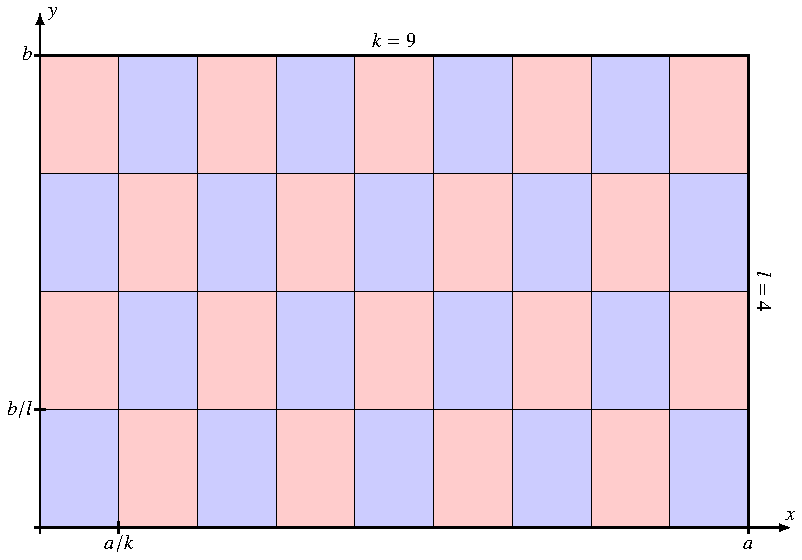
\includegraphics{chapters/090-pde/images/rechteck.pdf}
\caption{Vorzeichen und Knotenlinie der Eigenfunktion
$U_{kl}(x,y)$ des Laplace-Operators auf dem Rechteck $(0,a)\times (0,b)$.
In den blauen Rechtecken gilt $U_{kl}(x,y)>0$ in den roten gilt
$U_{kl}(x,y)<0$.
die vertikalen und horizontalen schwarzen Linien sind Knotenlinien
der Eigenfunktion, ihre $x$-Koordinaten sind Vielfache von $a/k$,
die $y$-Koordinaten sind Vielfache von $b/l$.
\label{buch:pde:rechteck:fig:knoten}}
\end{figure}
Die Lösungen $U_{kl}(x,y)$ aus \eqref{buch:pde:rechteck:eqn:ukl}
sind Lösungen der ursprünglichen Differentialgleichung 
$\Delta U=-\lambda^2 U$.
Durch Einsetzen lassen sich jetzt auch die Eigenwerte bestimmen:
\begin{align*}
\Delta U_{kl}(x,y)
&=
-\frac{k^2\pi^2}{a^2} \sin\frac{k\pi}{a}x\cdot \sin\frac{k\pi}{b}y
-\frac{l^2\pi^2}{b^2} \sin\frac{k\pi}{a}x\cdot \sin\frac{k\pi}{b}y
=
-\biggl(\frac{k^2\pi^2}{a^2}+\frac{l^2\pi^2}{b^2}\biggr) U_{kl}(x,y)
\end{align*}
Die Eigenfrequenzen einer rechtecking schwingenden Membran sind also
\[
\lambda
=
\sqrt{
\frac{k^2\pi^2}{a^2}+\frac{l^2\pi^2}{b^2}
}.
\]
Die Vorzeichen und die Knotenlinien der $U_{kl}(x,y)$ des
Eigenwertproblems ist in Abbildung~\ref{buch:pde:rechteck:fig:knoten}
dargestellt.

%
% kreis.tex
%
% (c) 2021 Prof Dr Andreas Müller, OST Ostschweizer Fachhochschule
%
\section{Kreisförmige Membran
\label{buch:pde:section:kreis}}
In diesem Abschnitt soll die Differentialgleichung einer kreisförmigen
Membran mit Hilfe der Separationsmethode gelöst werden.
Dabei werden die Bessel-Funktionen als Lösungsfunktionen 
auftreten und die Eigenfrequenzen werden durch ihre Nullstellen
berechnet.

\subsection{Differentialgleichung und Randbedingung}
Die Wellengleichung auf einem Kreisgebiet mit Radius $r_0$ 
lässt sich am besten mit Hilfe von Polarkoordinaten $(r,\varphi)$
ausdrücken.
Gesucht ist also eine Funktion $u(t,r,\varphi)$ gesucht, wobei
$0\le r<r_0$ und $0\le \varphi\le 2\pi$.
Die Funktion muss eine Lösung der Wellengleichung
\[
\frac{1}{c^2}\frac{\partial^2u}{\partial t^2} = \Delta u
\]
sein.

Der Laplace-Operator hat in Polarkoordinaten die Form
\begin{equation}
\Delta
=
\frac{\partial^2}{\partial r^2}
+
\frac1r
\frac{\partial}{\partial r}
+
\frac{1}{r 2}
\frac{\partial^2}{\partial\varphi^2}.
\label{buch:pde:kreis:laplace}
\end{equation}
Die Differentialgleichung ist 
\[
\frac{1}{c^2} \frac{\partial^2 u}{\partial t^2}
=
\Delta u.
\]
Die Separation der Zeit führt auf die Eigenwertgleichung
\[
\Delta U(r,\varphi) = -\lambda^2 U(r,\varphi)
\]
für eine Funktion, die nur von $r$ und $\varphi$ abhängt.

Die Randbedingungen besagen, dass $u(t,r_0,\varphi)=0$ für $t>0$.
Dies bedeutet für die Funktion $U(r,\varphi)$, dass
$U(r_0,\varphi)=0$ sein muss für alle $\varphi$.

Die Bedingungen an $U$ reichen aber nicht ganz.
Alle Koordinaten $(0,\varphi)$ bezeichnen ja gleichermassen
den Nullpunkt des Koordinatensystems, es muss also auch sichergestellt
sein, dass $U(0,\varphi)$ für alle $\varphi$ den gleichen Wert gibt.

\subsection{Separation}
Das Eigenwertproblem $\Delta U=-\lambda^2 U$ soll jetzt in Polarkoordinaten
separiert werden.
Dazu schreiben wir die Lösung als
\[
U(r,\varphi)
=
R(r)\cdot \Phi(\varphi).
\]
Die Randbedingungen an $U$ werden zu $R(r_0)=0$.

Im Ursprung des Koordinatensystems ist die Randbedingung etwas
komplizierter.
Wenn $R(0)=0$ ist, dann ist sichergestellt, dass
$U(0,\varphi)=R(0)\Phi(\varphi)0$ ist, dass also der Wert unabhängig
ist von $\varphi$.
Wenn aber $R(0)\ne 0$ ist, dann kann die geforderte Unabhängigkeit
von $\varphi$ nur erfüllt werden, wenn $\Phi(\varphi)$ konstant ist.
Da die Funktion aber auch noch differenzierbar sein soll, darf es
an der Stelle $r=0$ keine ``Spitze'' geben, die Ableitung $R'(0)$
muss also auch $=0$ sein.
% XXX Evtl Bild zur Illustration dieses Problems

Die Differntialgleichungen wird mit der Form~\eqref{buch:pde:kreis:laplace}
des Laplace-Operators
\[
\Delta U
=
R''(r) \Phi(\varphi)
+
\frac1r R'(r)\Phi(\varphi)
+
\frac{1}{r^2} R(r)\Phi''(\varphi)
=
-\lambda^2
R(r)\Phi(\varphi)
\]
Nach Division durch die rechte Seite erhalten wir
\[
\frac{R''(r)}{R(r)}
+
\frac1r \frac{R'(r)}{R(r)}
+
\frac{1}{r^2} \frac{\Phi''(\varphi)}{\Phi(\varphi)}
=
-\lambda^2
\]
Im letzten Term auf der linken Seite kommen die Variablen $r$ und $\varphi$
gemischt vor, man muss also die Gleichung erst mit $r^2$ multiplizieren,
bevor man sie in 
\[
\frac{r^2R''(r)+rR'(r)+\lambda^2 r^2R(r)}{R(r)}
=
-\frac{\Phi''(\varphi)}{\Phi(\varphi)}
\]
separieren kann.
Die beiden Seiten sind also konstant, wir nennen die gemeinsame
Konstanten $\mu^2$, das vereinfacht die Lösung der Gleichung
für $\Phi(\varphi)$.

Die Gleichung für $\Phi$ hat für $\mu\ne 0$ die Lösungen
\begin{align*}
\Phi(\varphi) &= \cos\mu\varphi
\text{und}\qquad
\Phi(\varphi) &= \sin\mu\varphi.
\end{align*}
Die Lösung muss aber auch stetig sein, d.~h.~es muss $\Phi(0)=\Phi(2\pi)$
gelten.
Dies ist nur möglich, wenn $\mu$ eine ganze Zahl ist.

Für $\mu=0$ hat das charakteristische Polynome eine doppelte Nullstelle,
die allgemeine Lösung lautet daher
\[
\Phi(\varphi)= C \varphi + D.
\]
Die Funktion $\Phi$ muss aber auch stetig sein, d.~h.~$\Phi(0)=\Phi(2\pi)$,
das ist mit $C\ne 0$ nicht möglich, somit kommt für $\mu=0$ nur die
Lösung $\Phi(\varphi)=D$ in Frage.

Die Gleichung für $R(r)$ wird jetzt
\begin{equation}
r^2R''(r) + rR'(r)+(\lambda^2 r^2-\mu^2)R(r)
=
0.
\label{buch:pde:kreis:Rdgl}
\end{equation}
Bis auf den Faktor $\lambda^2$ ist dies eine Besselsche Differentialgleichung.

\subsection{Umformung in eine Besselsche Differentialgleichung}
Die Funktion $y(x) = J_\mu(sx)$ hat die Ableitungen
\begin{align*}
y'(x) &= sJ'_mu(sx)      
\\
y''(x) &= s^2J''_\mu(sx)
\end{align*}
Setzt man dies in die Besselsche Differentialgleichung für $J_\mu$ an
der Stelle $sx$ ein, erhält man
\[
s^2x^2 J''_\mu(sx) + sx J'_\mu(sx) + (s^2x^2 -\mu^2) J_\mu(sx) = 0.
\]
Die Differentialgleichung \eqref{buch:pde:kreis:Rdgl} der Funktion $R(r)$
wird also gelöst von den Funktionen $R(r) = J_\mu(\lambda r)$.

\subsection{Eigenfrequenzen}
Im vorangegangenen Abschnitt haben wir gefunden, dass die Lösungen
für $R(r)$ die Funktionen $J_\mu(\lambda r)$ sind.
Bis jetzt haben wir aber nicht nachgeprüft, dass die Randbedingung
eingehalten wird. 
Diese ist erfüllt, $R(r_0)=0$ ist.
Es muss also
$J_\mu(\lambda r_0)=0$ sein, oder $\lambda r_0$ muss eine
Nullstelle von $J_{\mu}$ sein.
Bezeichnen wir die Nullstellen von $J_\mu$ mit $j_{\mu k}$, wobei $k$
eine natürliche Zahl ist, dann muss
\[
\lambda = \frac{j_{\mu k}}{r_0}
\]
sein.
Die Eigenfrequenzen der kreisförmigen Membran werden also im Wesentlichen
durch die Nullstellen der Bessel-Funktionen gegeben.

Zu jedem ganzzahligen $\mu$ gibt es also eine Folge $j_{\mu k}/r_0$  von
Eigenfrequenzen. 
Die Lösungen mit Index $k$ der Differentialgleichung mit Index $k$ hat
die Form
\[
U_{\mu k}(r,\varphi)
=
C \cos(\mu \varphi+\delta)
J_{\mu}\biggl(
\frac{j_{\mu k}}{r_0}r
\biggr)
\]
Der Faktor $J_{\mu}$ hat $k$ weitere Nullstellen für Radien $r<r_0$,diese
gehören zu kreisförmigen Knotenlinien der Membran, dort bewegt sie sich
nicht.
Der Faktor $\cos(\mu\varphi+\delta)$ hat $2\mu$ Nullstellen im Intervall
$[0,2\pi)$, es gibt also noch zusätzlich $\mu$ diametrale Knotenlinien.
Nur für $\mu=0$ gibt es Lösungen, die keine radialen Knotenlinien haben,
da in diesem Fall $\Phi$ eine konstante Funktion sein muss.

\begin{table}
\centering
\begin{tabular}{|>{$}c<{$}|>{$}r<{$}|>{$}r<{$}|>{$}r<{$}|>{$}r<{$}|>{$}r<{$}|>{$}r<{$}|>{$}r<{$}|>{$}r<{$}|}
\hline
 k & \mu = 0 & \mu = 1 & \mu = 2 & \mu = 3 & \mu = 4 & \mu = 5 & \mu = 6 & \mu = 7 \\
\hline
 0 &   2.4048& 0\phantom{.0000}& 0\phantom{.0000}& 0\phantom{.0000}& 0\phantom{.0000}& 0\phantom{.0000}& 0\phantom{.0000}& 0\phantom{.0000}\\
 1 &   5.5201&   3.8317&   5.1356&   6.3802&   7.5883&   8.7715&   9.9361&  11.0864\\
 2 &   8.6537&   7.0156&   8.4172&   9.7610&  11.0647&  12.3386&  13.5893&  14.8213\\
 3 &  11.7915&  10.1735&  11.6198&  13.0152&  14.3725&  15.7002&  17.0038&  18.2876\\
 4 &  14.9309&  13.3237&  14.7960&  16.2235&  17.6160&  18.9801&  20.3208&  21.6415\\
 5 &  18.0711&  16.4706&  17.9598&  19.4094&  20.8269&  22.2178&  23.5861&  24.9349\\
 6 &  21.2116&  19.6159&  21.1170&  22.5827&  24.0190&  25.4303&  26.8202&  28.1912\\
 7 &  24.3525&  22.7601&  24.2701&  25.7482&  27.1991&  28.6266&  30.0337&  31.4228\\
 8 &  27.4935&  25.9037&  27.4206&  28.9084&  30.3710&  31.8117&  33.2330&  34.6371\\
 9 &  30.6346&  29.0468&  30.5692&  32.0649&  33.5371&  34.9888&  36.4220&  37.8387\\
 10 &  33.7758&  32.1897&  33.7165&  35.2187&  36.6990&  38.1599&  39.6032&  41.0308\\
\hline
\end{tabular}

\caption{Nullstellen der Bessel-Funktionen
\label{buch:pde:kreis:table:besselzeros}}
\end{table}

\begin{figure}
\centering
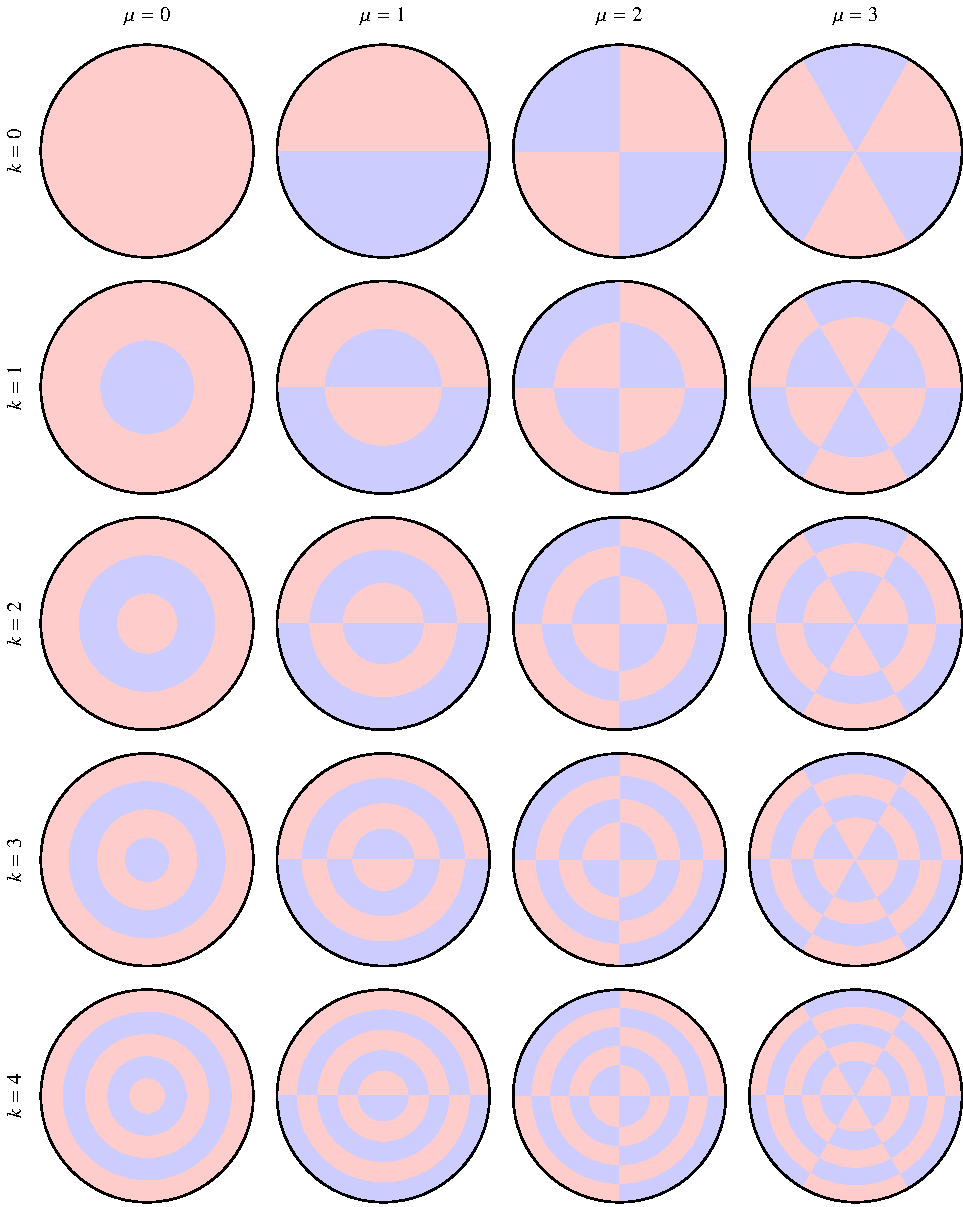
\includegraphics[width=\textwidth]{chapters/090-pde/bessel/pauke.pdf}
\caption{Vorzeichen der Lösungsfunktionen und Knotenlinien
für verschiedene Werte von $\mu$ und $k$.
Die Bereiche, in denen die Lösungsfunktion positiv sind, ist 
rot dargestellt, die negativen Bereiche blau.
In jeder Darstellung gibt es genau $k+\mu$ Knotenlinien.
Die Radien der kreisförmigen Knotenlinien müssen aus den Nullstellen
der Besselfunktionen berechnet werden.
\label{buch:pde:kreis:fig:pauke}}
\end{figure}

%
% kugel.tex
%
% (c) 2021 Prof Dr Andreas Müller, OST Ostschweizer Fachhochschule
%
\section{Kugelfunktionen
\label{buch:pde:section:kugel}}
Kugelsymmetrische Probleme können oft vorteilhaft in Kugelkoordinaten
beschrieben werden.
Die Separationsmethode kann auf partielle Differentialgleichungen
mit dem Laplace-Operator angewendet werden.
Die daraus resultierenden gewöhnlichen Differentialgleichungen führen
einerseits auf die Laguerre-Differentialgleichung für den radialen
Anteil sowie auf Kugelfunktionen für die Koordinaten der
geographischen Länge und Breite.

\subsection{Kugelkoordinaten}
Wir verwenden Kugelkoordinaten $(r,\vartheta,\varphi)$, wobei $r$
der Radius ist, $\vartheta$ die geographische Breite gemessen vom
Nordpol der Kugel und $\varphi$ die geographische Breite.
Der Definitionsbereich für Kugelkoordinaten ist
\[
\Omega
=
\{(r,\vartheta,\varphi)
\;|\;
r\ge 0\wedge 
0\le \vartheta\le \pi\wedge
0\le \varphi< 2\pi
\}.
\]
Die Entfernung eines Punktes von der $z$-Achse ist $r\sin\vartheta$.
Daraus lassen sich die karteischen Koordinaten eines Punktes mit Hilfe
von
\[
\begin{pmatrix}x\\y\\z\end{pmatrix}
=
\begin{pmatrix}
r\cos\vartheta\\
r\sin\vartheta\cos\varphi\\
r\sin\vartheta\sin\varphi
\end{pmatrix}.
\]
Man beachte, dass die Punkte auf der $z$-Achse keine eindeutigen
Kugelkoordinaten haben.
Sie sind charakterisiert durch $r\sin\vartheta=0$, was $\cos\vartheta=\pm1$
impliziert.
Entsprechend führen alle Werte von $\varphi$ auf den gleichen Punkt
$(0,0,\pm r)$.

\subsection{Der Laplace-Operator in Kugelkoordinaten}
Der Laplace-Operator in Kugelkoordinaten lautet
\begin{align}
\Delta
&=
\frac{1}{r^2} \frac{\partial}{\partial r}r^2\frac{\partial}{\partial r}
+
\frac{1}{r^2\sin\vartheta}\frac{\partial}{\partial\vartheta}
\sin\vartheta\frac{\partial}{\partial\vartheta}
+
\frac{1}{r^2\sin^2\vartheta}\frac{\partial^2}{\partial\varphi^2}.
\label{buch:pde:kugel:laplace1}
\intertext{Dies kann auch geschrieben werden als}
&=
\frac{\partial^2}{\partial r^2}
+
\frac{2}{r}\frac{\partial}{\partial r}
+
\frac{1}{r^2\sin\vartheta}\frac{\partial}{\partial\vartheta}
\sin\vartheta\frac{\partial}{\partial\vartheta}
+
\frac{1}{r^2\sin^2\vartheta}\frac{\partial^2}{\partial\varphi^2}
\label{buch:pde:kugel:laplace2}
\intertext{oder}
&=
\frac{1}{r}
\frac{\partial^2}{\partial r^2} r
+
\frac{1}{r^2\sin\vartheta}\frac{\partial}{\partial\vartheta}
\sin\vartheta\frac{\partial}{\partial\vartheta}
+
\frac{1}{r^2\sin^2\vartheta}\frac{\partial^2}{\partial\varphi^2}.
\label{buch:pde:kugel:laplace3}
\end{align}
Dabei ist zu berücksichtigen, dass mit der Notation gemeint ist,
dass ein Ableitungsoperator auf alles wirkt, was rechts im gleichen
Term steht.
Der Operator
\[
\frac{1}{r}
\frac{\partial^2}{\partial r^2}r
\quad\text{wirkt daher als}\quad
\frac{1}{r}
\frac{\partial^2}{\partial r^2}rf
=
\frac{1}{r}
\frac{\partial}{\partial r}\biggl(f + r\frac{\partial f}{\partial r}\biggr)
=
\frac{1}{r}
\frac{\partial f}{\partial r}
+
\frac{1}{r}
\frac{\partial f}{\partial r}
+
\frac{\partial^2f}{\partial r^2}.
=
\frac{2}{r}\frac{\partial f}{\partial r}
+
\frac{\partial^2f}{\partial r^2},
\]
was die Äquivalenz der beiden Formen
\eqref{buch:pde:kugel:laplace2}
und
\eqref{buch:pde:kugel:laplace3}
rechtfertigt.
Auch die Äquivalenz mit
\eqref{buch:pde:kugel:laplace1}
kann auf ähnliche Weise verstanden werden.

Die Herleitung dieser Formel ist ziemlich aufwendig und soll hier
nicht dargestellt werden.
Es sei aber darauf hingewiesen, dass sich für $\vartheta=\frac{\pi}2$ 
wegen $\sin\vartheta=\sin\frac{\pi}2=1$
der eingeschränkte Operator
\[
\Delta
= 
\frac{1}{r^2}\frac{\partial }{\partial r} r^2\frac{\partial}{\partial r}
+
\frac{1}{r^2}\frac{\partial^2}{\partial\varphi^2}
\]
ergibt.
Wendet man wie oben die Produktregel auf den ersten Term an, entsteht die
Form
\[
\frac{\partial^2}{\partial r^2}
+
\frac{2}{r}
\frac{\partial}{\partial r}
+
\frac{1}{r^2}\frac{\partial^2}{\partial\varphi^2}
\]
die {\em nicht} übereinstimmt mit dem Laplace-Operator in 
Polarkoordinaten~\eqref{buch:pde:kreis:laplace}.
Der Unterschied rührt daher, dass der Laplace-Operator die Krümmung
der Koordinatenlinien berücksichtigt, in diesem Fall der Meridiane.

\subsection{Separation}
In Abschnitt~\ref{buch:pde:subsection:eigenwertproblem}
wurde bereits gzeigt, wie die Wellengleichung
\[
\frac{1}{c^2}
\frac{\partial^2 U}{\partial t^2}
-\Delta U
=
0
\]
durch Separation der Zeit auf ein Eigenwertproblem für eine
Funktion $u$ reduziert werden kann, die nur von den Ortskoordinaten
abhängt.
Es geht also nur noch darum, dass Eigenwertproblem
\[
\Delta u = -\lambda^2 u
\]
mit geeigneten Randbedingungen zu lösen.
Dazu gehören einerseits eventuelle Gebietsränder, die im Moment
nicht interessieren.
Andererseits muss sichergestellt sein, dass die Lösungsfunktionen
stetig und differentierbar sind an den Orten, wo das Koordinatensystem
singulär ist.
So müssen $u(r,\vartheta,\varphi)$ $2\pi$-periodisch in $\varphi$ sein.
% XXX Ableitungen

\subsubsection{Separation des radialen Anteils}
Für das Eigenwertproblem verwenden wir den Ansatz
\[
u(r,\vartheta,\varphi)
=
R(r) \Theta(\vartheta) \Phi(\varphi),
\]
den wir in die Differentialgleichung einsetzen.
So erhalten wir
\[
\biggl(\frac{1}{r^2}R''(r)+\frac{2}{r}R'(r) \biggr)
\Theta(\vartheta)\Phi(\varphi)
+
R(r)
\frac{1}{r^2\sin\vartheta}
\frac{\partial}{\partial\vartheta}(\sin\vartheta \Theta'(\vartheta))
\Phi(\varphi)
+
R(r)\Theta(\vartheta)
\frac{1}{r^2\sin\vartheta} \Phi''(\varphi)
=
-\lambda^2 R(r)\Theta(\vartheta)\Phi(\varphi).
\]
Die Gleichung lässt sich nach Multiplikation mit $r^2$ und
Division durch $u$ separieren in 
\begin{equation}
\frac{R''(r)+2rR'(r)+\lambda^2r^2}{R(r)}
+
\frac{1}{\Theta(\vartheta) \sin\vartheta}
\frac{\partial}{\partial\vartheta}\sin\vartheta\Theta'(\vartheta)
+
\frac{1}{\sin^2\vartheta}\frac{\Phi''(\varphi)}{\Phi(\varphi)}
=
0
\label{buch:pde:kugel:separiert2}
\end{equation}
Der erste Term hängt nur von $r$ ab, die anderen nur von $\vartheta$ und
$\varphi$, daher muss der erste Term konstant sein.
Damit ergbit sich für den Radialanteil die gewöhnliche Differentialgleichung
\[
R''(r) + 2rR'(r) +\lambda^2 r^2 = \mu^2 R(r),
\]
die zum Beispiel mit der Potenzreihenmethode gelöst werden kann.
Sie kann aber durch eine geeignete Substition nochmals auf die
Laguerre-Differentialgleichung reduziert werden, wie in
Kapitel~\ref{chapter:laguerre} dargelegt wird.

\subsubsection{Kugelflächenanteil}
Für die Separation der verbleibenden winkelabhängigen Teile muss die
Gleichung
\[
\frac{1}{\Theta(\vartheta) \sin\vartheta}
\frac{\partial}{\partial\vartheta}\sin\vartheta\Theta'(\vartheta)
+
\frac{1}{\sin^2\vartheta}\frac{\Phi''(\varphi)}{\Phi(\varphi)}
=
-\mu^2
\]
mit $\sin^2\vartheta$ multipliziert werden, was auf
\[
\frac{\sin\vartheta}{\Theta(\vartheta)}
\frac{\partial}{\partial\vartheta}\sin\vartheta\Theta'(\vartheta)
+
\frac{\Phi''(\varphi)}{\Phi(\varphi)}
=
-\mu^2\sin^2\vartheta
\quad\Rightarrow\quad
\frac{\sin\vartheta}{\Theta(\vartheta)}
\frac{\partial}{\partial\vartheta}\sin\vartheta\Theta'(\vartheta)
+
\mu^2\sin^2\vartheta
=
-
\frac{\Phi''(\varphi)}{\Phi(\varphi)}
\]
führt.
Die linke Seite der letzten Gleichung hängt nur von $\vartheta$
ab, die rechte nur von $\varphi$, beide Seiten müssen daher
konstant sein, wir bezeichnen diese Konstante mit $\alpha^2$.
So ergibt sich die Differentialgleichung
\[
\alpha^2
=
-\frac{\Phi''(\varphi)}{\Phi(\varphi)}
\]
für die Abhängigkeit von $\varphi$, mit der allgemeinen Lösung
\[
\Phi(\varphi)
=
A\cos\alpha \varphi
+
B\sin\alpha \varphi.
\]
Die Randbedingungen verlangen, dass $\Phi(\varphi)$ eine $2\pi$-periodische
Funktion ist, was genau dann möglich ist, wenn $\alpha=m$ ganzzahlig ist.
Damit ergibt sich für die $\vartheta$-Abhängigkeit die Differentialgleichung
\begin{equation}
\frac{\sin\vartheta}{\Theta(\vartheta)}
\frac{\partial}{\partial\vartheta}\sin\vartheta\Theta'(\vartheta)
+
\mu^2\sin^2\vartheta
=
m^2.
\label{buch:pde:kugel:eqn:thetaanteil}
\end{equation}

\subsubsection{Abhängigkeit von $\vartheta$}
Die Differentialgleichung~\eqref{buch:pde:kugel:eqn:thetaanteil}
ist etwas unhandlich, daher verwenden wir die Substitution $z=\cos\vartheta$,
um die trigonometrischen Funktionen los zu werden.
Wegen
\[
\frac{dz}{d\vartheta} = -\sin\vartheta =-\sqrt{1-z^2}
\]
können die Ableitungen nach $\vartheta$ auch durch Ableitungen nach $z$
ausgedrückt werden.
Wir schreiben dazu $Z(z)=\Theta(\vartheta)$ und berechnen 
\[
\Theta'(\vartheta)
=
\frac{d\Theta}{d\vartheta}
=
\frac{dZ}{dz}\frac{dz}{d\vartheta}
=
-
\sqrt{1-z^2}
Z'(z).
\]
Dies bedeutet auch, dass
\[
\sin\vartheta\frac{d}{d\vartheta}
=
-
(1-z^2)\frac{d}{dz},
\]
damit lässt sich die Differentialgleichung für $\Theta(\vartheta)$ umschreiben
in eine Differentialgleichung für $Z(z)$, nämlich
\[
(1-z^2)\frac{d}{dz}(1-z^2)\frac{d}{dz} Z(z)
+
\mu^2
(1-z^2)
Z(z)
=
m^2
Z(z).
\]
Indem man die Ableitung im ersten Term mit Hilfe der Produktregel
ausführt, kann man die Gleichung
\[
(1-z^2)\biggl(
-2zZ'(z) + (1-z^2)Z''(z)
\biggr)
+
\mu^2(1-z^2)Z(z)
=
-m^2 Z(z)
\]
bekommen.
Division durch $1-z^2$ ergibt die
{\em Legendre-Differentialgleichung}
\begin{equation}
(1-z^2)Z''(z)
-2zZ'(z)
+
\biggl(
\mu^2 - \frac{m^2}{1-z^2}
\biggr)
Z(z)
=
0.
\label{buch:pde:kugel:eqn:legendre-dgl}
\end{equation}
Eine Diskussion der Lösungen dieser Differentialgleichung erfolgt im
Kapitel~\ref{chapter:kugel}.

\subsection{Kugelfunktionen}
Die Legendre-Differentialgleichung~\eqref{buch:pde:kugel:eqn:legendre-dgl}
hat Lösungen für Werte von $\mu$ derart, dass $\mu^2=l(l+1)$ für natürliche
Zahlen $l$.
Die Lösungen sind sogar Polynome, die wir mit $P_l^{(m)}(z)$ 
bezeichnen, dabei ist $m$ eine ganze Zahl mit $-l\le m\le l$.
Die Funktionen $P_l^{(m)}(\cos\vartheta)e^{im\varphi}$ 
sind daher alle Lösungen des von $\vartheta$ und $\varphi$
abhängigen Teils der Lösungen des Eigenwertproblems.
Mit einer geeigneten Normierung kann man zudem eine Familie von
bezüglich des Skalarproduktes
\[
\langle f,g\rangle_{S^2}
=
\int_{-\pi}^{\pi}
\int_{0}^{\pi}
\overline{f(\vartheta,\varphi)}
g(\vartheta,\varphi)
\sin\vartheta
\,d\vartheta
\,d\varphi
\]
orthonormiete Funktionen auf der Kugeloberfläche erhalten, die
man normalerweise als 
\[
Y_{lm}(\vartheta,\varphi)
=
\frac{1}{\sqrt{2\pi}}
\sqrt{
\frac{2l+1}{2}\cdot
\frac{(l-m)!}{(l+m)!}
}
P_{l}^{(m)}(\cos\vartheta)e^{im\varphi}
\]
bezeichnet.







\section*{Übungsaufgaben}
\rhead{Übungsaufgaben}
\aufgabetoplevel{chapters/090-pde/uebungsaufgaben}
\begin{uebungsaufgaben}
\uebungsaufgabe{901}
%\uebungsaufgabe{1}
\end{uebungsaufgaben}

